
\begin{frame}
    \frametitle{Enhanced BBI platform}
%    Schéma
    \begin{textblock*}{60mm}(48mm, 16mm)
        \includegraphics[width=\textwidth]{model2ProbeManuscrit.pdf}
    \end{textblock*}
%   Flèche gauche
    \begin{textblock*}{1mm}(28mm, 24mm)
        \begin{tikzpicture}
                \draw[-Latex, black, line width=0.5mm] (0, 0) -| (-3, -2.35);
            \end{tikzpicture}
    \end{textblock*}
%   Flèche droite
    \begin{textblock*}{1mm}(99mm, 35.0mm)
        \begin{tikzpicture}
            \draw[-Latex, black, line width=0.5mm] (0, 0) -| (2.9, -1.2);
        \end{tikzpicture}
    \end{textblock*}
%    Courant
    \begin{textblock*}{60mm}(98mm, 49mm)
        \includegraphics[width=\textwidth]{S2G.pdf}
    \end{textblock*}
%    Pulse
    \begin{textblock*}{60mm}(2mm, 49mm)
        \includegraphics[width=\textwidth]{S2P.pdf}
    \end{textblock*}
%    impMatchGen
    \begin{textblock*}{28mm}(67mm, 51mm)
        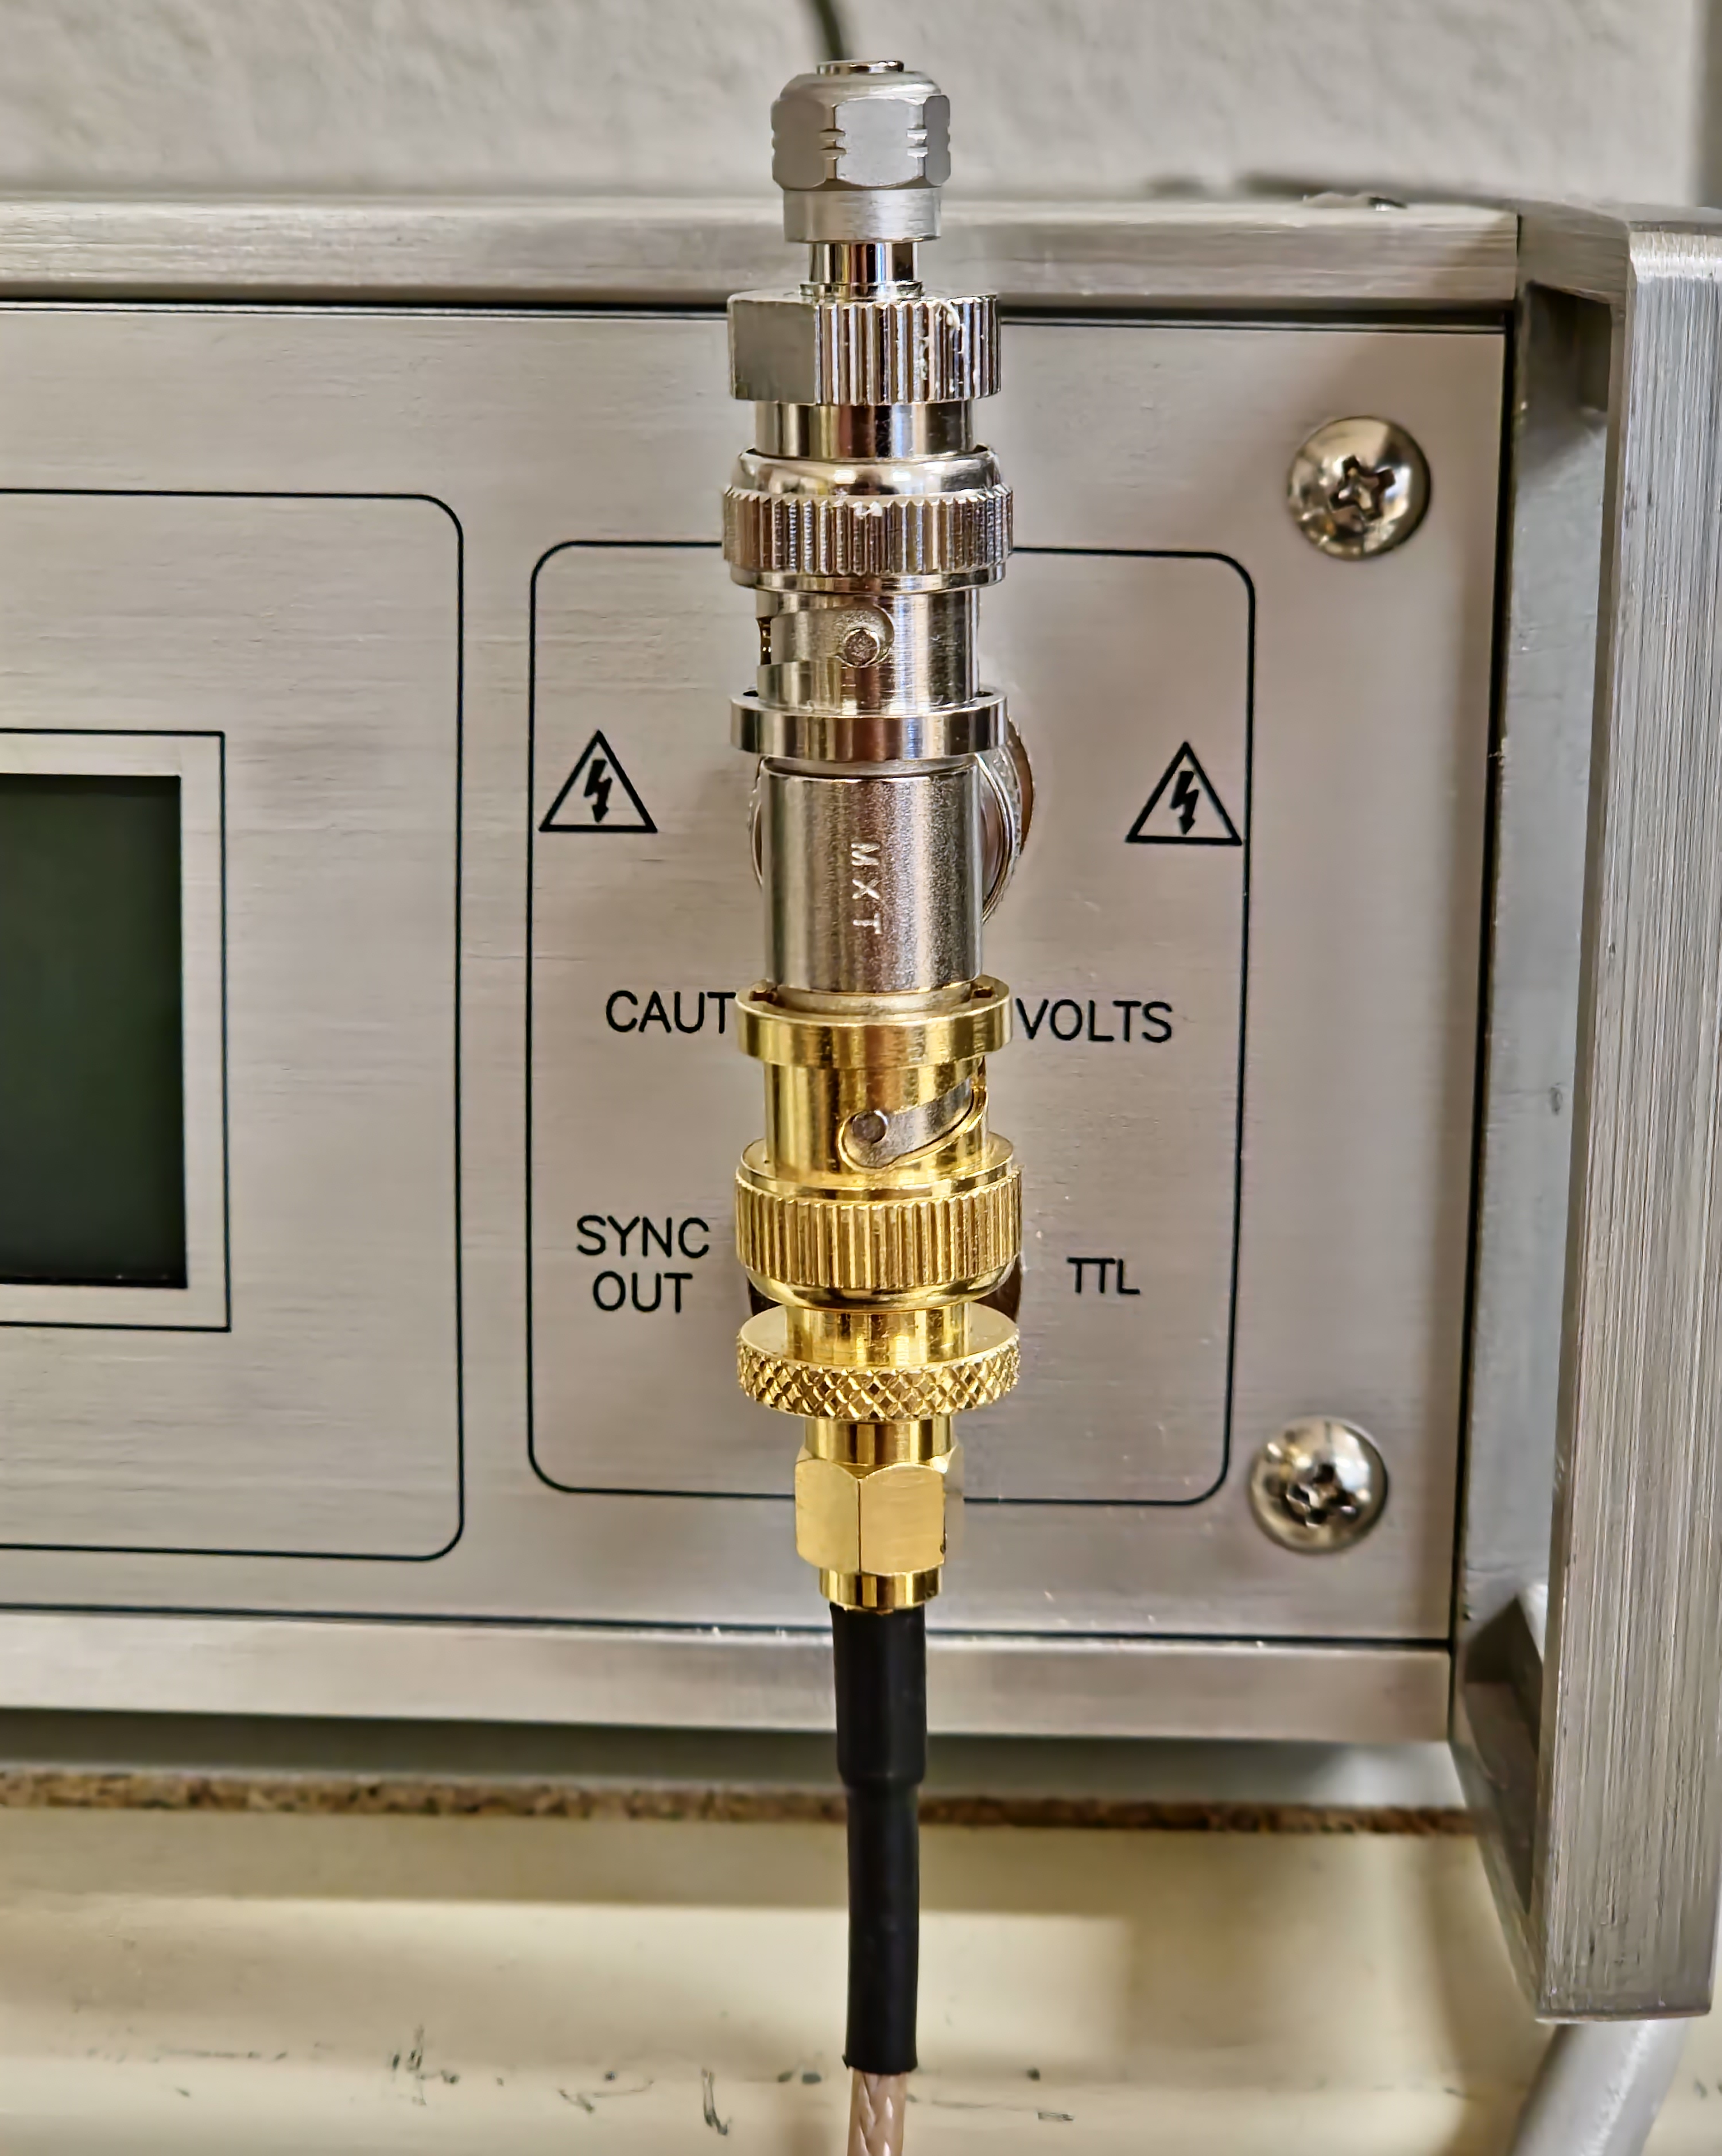
\includegraphics[width=\textwidth]{impMatchPicture.jpg}
    \end{textblock*}
%    cercle image
    \begin{textblock*}{1mm}(75.3mm, 50mm)
        
\begin{tikzpicture}
            \draw[line width=0.5mm, color=red] circle (0.3);
        \end{tikzpicture}
    \end{textblock*}
%   Flèche image
    \begin{textblock*}{1mm}(66mm, 34mm)
        \begin{tikzpicture}
            \draw[-Latex, red, line width=0.5mm] (0, 0) |- (0.8, -1.9);
        \end{tikzpicture}
    \end{textblock*}
\end{frame}
